\section{Introduction}

Solid fueled nuclear reactors differ from liquid fueled reactors with respect 
to many physical domains including neutronics, thermal hydraulics, and 
materials performance. Accordingly, liquid fueled reactors challenge the 
capabilities of conventional computational tools designed for modeling and simulating 
the physics of solid fueled reactors. 

These challenges compound one another in numerical simulations that model the 
coupling between physics, particularly in liquid fueled reactors in which the 
fuel \emph{circulates}. In such reactors, neutron kinetics, fuel depletion, 
heat transport, and fluid flow couple together much more tightly, stiffening 
the interdependent system of \glspl{PDE} driving reactor behavior.
While solid fueled reactor simulation can accurately couple 
neutronics and thermal hydraulics through operator splitting techniques and 
loose coupling, such approaches cannot capture the tightly coupled 
multiphysics of reactors with circulating liquid fuel.

\section{Liquid vs. Solid Fuel}
Differences between liquid and solid fueled designs arise primarily from the 
mobility of the dissolved fuel. This feature impacts neutronics, thermal 
hydraulics, and the relationship between them. In particular, modeling and 
simulating time dependent reactor dynamics can require new methods when coupling 
neutron kinetics, feedbacks, and depletion dynamics with fuel expansion, flow
dynamics, heat removal, and system safety. 

\subsection{Neutronic Differences}

In all liquid fueled molten salt reactors, salt movement directly impacts 
neutron kinetics and control through delayed neutron precursor movement. Since 
the fissionable material is dissolved in the fuel salt, isotopes produced by 
fission also move congruously with the salt. Reactor controllability hinges upon 
delayed neutron precursors, which contribute to $\beta_{eff}$, the delayed 
neutron precursor fraction.

Circulating fuels can additionally be reprocessed during reactor operation. 
Thus, fuel composition in liquid fueled reactors not only varies with in-core 
transmutation, but also through out-of-core chemical extraction, gas sparging, mechanical 
filtering, and other methods. For example, several fission products selectively 
precipitate onto nickel surfaces in fluoride salt, as documented in 
\cite{engel_conceptual_1980}, allowing those to be removed when the fuel salt is 
circulated out of the core, reducing unwanted neutron absorption. 
These dynamics occur on fast timescales (minutes) if the fuel is reprocessed 
``online'' or on slower, discrete timescales if the design involves processing 
in batches.

Very long fuel residence times in circulating, liquid fueled reactors also 
presents a challenge regarding depletion dynamics. In contrast to legacy 
reactors, material damage to the fuel does not limit burnup. Instead, corrosion 
and fast neutron damage to other structures (e.g.  graphite moderation 
structures) limit burnup.  If those structures are protected (as in 
\cite{engel_conceptual_1980}) reactor operation can continue without opening 
the vessel for thirty or more years. The buildup and transmutation of fission 
products in the vessel during that time impacts reaction rates over the course 
of years or decades. Computational tools to accurately characterise this 
depletion evolution must incorporate chemical processing logistics as well.

Additionally, fuel temperature reactivity feedback related to salt density is 
very strong in liquid fueled \glspl{MSR}. Though the fuel salt remains single phase, 
density variation with temperature impacts fuel isotope number densities, 
$N_i$, and corresponding reaction rates $\sigma_xN_i\Phi$, resulting in very 
strong fuel temperature feedbacks. For example, in fast-spectrum fluoride 
\glspl{MSR}, salt expansion contributes approximately half of the total 
temperature reactivity coefficient \cite{aufiero_monte_2017}.

\subsection{Thermal Hydraulic Differences}

In \gls{MSR} concepts, the fuel salt remains in a single, liquid phase throughout 
normal operation. 
And, in contrast to conventional reactors, \glspl{MSR} operate at near 
atmospheric pressures and very high temperatures, frequently with very high 
Prandtl number flow. Natural circulation in these 
fluids plays a strong role in reactor performance, and although many designs 
incorporate pumps to drive fuel circulation, some designs may rely on natural 
circulation driven flow instead.

Such single-phase flows can typically be modeled with the incompressible 
Navier-Stokes equations or a weakly compressible lattice-Boltzmann equation.  
However, in  startup, shutdown, off-normal operation, 
and accident scenarios, simulations may need to capture the solid and gaseous 
phases as well.

The gaseous phase must be considered because gaseous fission product isotopes 
appear in the liquid fuel during operation. As gaseous fission product 
inventory evolves, microbubbles may form when these gases coalesce. Aufiero et 
al. \cite{aufiero_monte_2017} recently showed significant impact to reactor 
neutronics from compressibility in the salt potentially introduced by such 
microbubbles. Since these microbubbles cannot be neglected in safety 
assessment, mass transport must be incorporated into any multiphysics 
assessment of liquid-fueled \glspl{MSR}.

In certain designs stationary flow vortices may develop as well, potentially 
causing the fuel salt in that location to overheat and evaporate. Such voiding 
can be avoided at the design stage if computational tools can accurately 
capture such vortical stagnation points in the flow. 

Finally, the solid phase may need to be considered when simulating ``freeze plugs,'' 
solidified salt which may block a channel. Some designs incorporate freeze as 
an intentional safety valve which melts at a high core temperature, allowing 
the core salt to drop into a dump tank or other safe configuration 
\cite{li_preliminary_2014}.  Transition into solid phase (freezing) is most 
likely to occur in small out-of-core fuel piping under off-normal scenarios. 

Toward validation of this software, new experimental flow loops (e.g.  
\cite{britsch_natural_2019}), promise to correct a dearth of experimental data 
regarding thermophysical properties for these salts and their natural 
circulation behavior.  

\subsection{Coupling Differences}

While loose coupling (e.g. operator splitting) can be sufficient for solid 
fueld reactors, tight interdependencies among neutronics and thermal 
hydraulics must be modeled as tightly or fully coupled. A fully coupled 
approach demands methods which are stable, parallelizable, and multi-scale. Common 
approximations in both thermal hydraulics and neutronics may need to be used 
with care. Specifically, methods which
neglect density variation (e.g. Boussinesq), rapidly changing isotopics (e.g. 
cross sections generated a single isotopic composition), or compressibility 
(Navier-Stokes), may fail to capture important coupled phenomena.

Additionally, simulation of time dependent multiphysics phenomena in \glspl{MSR} must 
handle neutronics concerns at many time scales such as density-driven 
temperature feedbacks, delayed neutron precursor drift, and composition changes 
due to online reprocessing. Multiphysics modeling must similarly handle thermal hydraulics concerns 
such as thermal expansion, compressibility due to fission gases, natural 
circulation, and evaporation or solidification of the fuel salt.

\section{Coupled Multiphysics Modeling}

Forward looking needs and challenges for modeling and simulation of any molten 
salt reactor will address separate neutronic and thermal hydraulic modeling 
challenges as well as unique issues with respect to coupling them.

\subsection{Current Tools}
With the inclusion of the \gls{MSR} among the Generation-IV reactor designs
\cite{gif_generation_2008,gif_generation_2015} and many new nuclear companies proposing both
liquid-fueled and solid-fueled commercial \gls{MSR} concepts
\cite{hyde_liquid_2015,leblanc_integral_2015,thorcon_-able_2017,scarlat_design_2014,transatomic_power_corporation_neutronics_2016}, 
corresponding tools for modeling and simulation of the coupled physics are in 
development internationally. 

Standard Monte Carlo \cite{leppanen_serpent_2015,werner_mcnp_2017} and deterministic 
\cite{rearden_scale:_2016} 
transport solvers capably handle static neutronic analysis of \glspl{MSR} 
However, time dependent kinetics and dynamics analysis cannot be achieved with 
conventional software. Toward this end, various efforts have extended or 
created custom tools which incorporate delayed neutron precursor drift. 
Some solutions have coupled \gls{CFD} with Monte Carlo, while others are built 
on software packages such as \gls{COMSOL} \cite{comsol_ab_comsol_2018} or 
\gls{MOOSE} \cite{gaston_physics-based_2015,gaston_parallel_2009} fundamentally designed 
for multiphysics coupling. 

In 2007, K\u{r}epel et al. extended the \gls{LWR}
diffusion code DYN3D to incorporate delayed neutron precursor drift and fission 
energy release directly into the mobile coolant. K\u{r}epel et al. demonstrated 
the resulting tool, DYN3D-MSR, via simulation of the \gls{MSRE} \cite{krepel_dyn3d-msr_2007}.
Soon thereafter, Kophazi et al. used iterative coupling between in-house
three-dimensional neutronic and one-dimensional heat conduction models DALTON
and THERM to analyze normal \gls{MSRE} operation as well as
channel-blocking-incident transients \cite{kophazi_development_2009}. The
Kophazi model added entrance effects of heat transfer coefficients as well as
thermal coupling between fuel channels through moderator heat conduction. 

More recently, Cammi et al. performed a 2D-axisymmetric single-channel analysis 
of the \gls{MSBR} using the commercial finite element package COMSOL 
Multiphysics \cite{cammi_multi-physics_2011}. That work directly solved for the 
fuel salt velocity field, used heterogeneous group constants in fuel and 
moderator regions, and employed the \gls{COMSOL} software package intrinsically 
designed for coupled multiphysics simulation.  Fiorina, Lathouwers, and their 
colleagues conducted a benchmarking exercise \cite{fiorina_modelling_2014} in 
which this Politecnico di Milano approach was expanded to a multi-channel model 
of the \gls{MSFR} and compared to code from the University of Delft 
\cite{de_zwaan_static_2007,van_der_linden_coupled_2012} based on the 
2009 DALTON/THERM iterative coupling approach in \cite{kophazi_development_2009}. 
These models showed good agreement for multiple accident transients. Meanwhile, 
leveraging lessons learned from these efforts resulted in a multiscale 
approach from Zanetti et al. in 2015 \cite{zanetti_geometric_2015} successfully 
combines high and low geometric fidelity for graphite-moderated \glspl{MSR}.

The most recent developments in this area leverage open frameworks such as 
the multiphysics \gls{MOOSE} framework \cite{gaston_physics-based_2015,gaston_parallel_2009} or 
the \gls{CFD} framework OpenFOAM\cite{weller_tensorial_1998}. In concert with the \gls{INL} \gls{MOOSE} 
framework, Lindsay et al. 
\cite{lindsay_introduction_2018,lindsay_moltres:_2018} developed and 
demonstrated a finite element based application, Moltres, with full coupling between 
multi-group diffusion neutronics with delayed neutron precursor drift and the Navier 
Stokes equations. Moltres is in continued active development \cite{huff_neutron_2018} at the 
University of Illinois alongside the helper utility SaltProc 
\cite{rykhlevskii_modeling_2018,rykhlevskii_online_2017} which simulates online fuel reprocessing via 
depletion with SERPENT2\cite{leppanen_serpent_2015}. The 
processing flow chart for SaltProc v.1.0 appears in Figure \ref{fig:saltproc}.

\begin{figure}[htbp]
        \begin{center}
                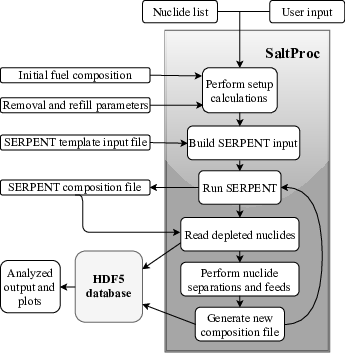
\includegraphics[width=0.5\textwidth]{saltproc_flowchart.png}
        \end{center}
        \caption{SaltProc couples to Serpent to add and remove specific isotopes from the core
        at the appropriate reprocessing intervals, mass rate, removal 
        efficiency to simulate fuel management. Figure reproduced from 
        \cite{rykhlevskii_modeling_2018,rykhlevskii_online_2017}.}
        \label{fig:saltproc} 
\end{figure}

Very recently, Aufiero et al. \cite{aufiero_development_2014} have begun to
approach transient simulations in the \gls{MSFR} within the finite volume
OpenFOAM \gls{CFD} toolkit \cite{weller_tensorial_1998}.  This approach
benefits from pre-implemented turbulence models available in the OpenFOAM
library and captures the full-core three-dimensional geometry of the reactor
primary circuit.  OpenFOAM \gls{CFD} has additionally been shown by Laureau et
al. \cite{laureau_transient_2017} to couple well with Transient Fission Matrix
neutronics within the \gls{MSFR}. This OpenFOAM coupling approach also enabled the 
first analysis of compressibility effects in the \gls{MSFR} by Aufiero et al. 
\cite{aufiero_monte_2017}. That work has been extended this year by Cervi et 
al., who incorporated modeling of a helium bubbling system envisioned for 
fission product removal in the \gls{MSFR} and assessed the impacts of that 
system on coupled thermal hydraulics and neutronics with respect to 
compressibility \cite{cervi_development_2019}. As shown in Figure 
\ref{fig:cervi}, reproduced from \cite{cervi_development_2019}, this simulation 
approach uses tight, but not full coupling, in order to incorporate the fidelity 
awarded by Monte Carlo neutronics.

\begin{figure}[htbp]
        \begin{center}
                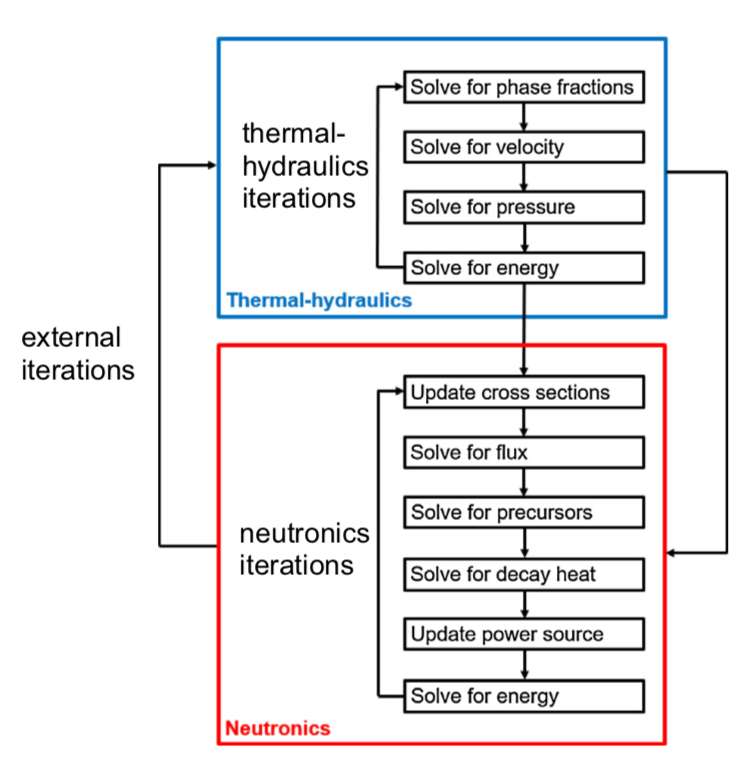
\includegraphics[width=0.5\textwidth]{./cervi_solver.png}
        \end{center}
        \caption{In this figure reproduced from \cite{cervi_development_2019}, 
        the structure of the coupling between Serpent and OpenFOAM is shown. 
        Picard iterations seek convergence of the thermal hydraulic solution, 
        then proceeds to solve the neutronics iterations.}
        \label{fig:cervi}
\end{figure}

Regarding thermal hydraulics, Leandro et al. \cite{leandro_thermal_2019} 
demonstrated \gls{MSRE} systems analysis with the \gls{NEAMS} \gls{SAM} module. 
Pressure drop predictions compared well to results from 
the \gls{MSRE} as well as RELAP5-3D simulation comparisons. Meanwhile, the existing \gls{MSR} 
multiphysics simulation tools mentioned in the previous section each capture some, but 
not all thermal hydraulic phenomena of importance in these reactors. 
With regard to thermal hydraulic modeling challenges, none of the current multiphysics 
tools capture one key operational safety challenge for these reactor 
types. Preliminary analysis indicates that serious local power density concerns 
may arise from \emph{stagnation points} in liquid fueled \glspl{MSR}.  When 
flow vortices arise in the core, fuel may become trapped in the vortical 
stagnation points, driving temperature increase which could damage reactor 
components or initiate boiling.  Quantifying the likelihood of stagnation 
points for the many operational states expected in these designs (e.g.  
load-following transients) is currently beyond the capability of existing 
molten salt multiphysics tools.

\subsection{Multiphysics Coupling Needs}

For stability, modeling multiphysics modeling and simulation approaches in 
\gls{MSR} regimes should use stable, fully coupled 
\gls{PDE} solver methods such as \gls{JFNK}. To capture the multi-scale nature 
of these systems simulations should incorporate adaptive meshing in 
both time and space.
For parallelizability, mesh handling methods such as domain decomposition must 
be available in the multiphysics framework or if the mesh is not domain 
decomposed, then the framework must scale well in memory. 
Applications built on the \gls{MOOSE} and \gls{COMSOL} frameworks both satisfy all 
of these requirements.  

\subsection{Conclusion}
To summarize, the main modeling and simulation needs for successful 
coupled multiphysics \gls{MSR} simulation stem from neutronic and thermal 
hydraulic behaviors unique to circulating molten salt fuels. While state-of-the-art \gls{MSR} 
simulation approaches now handle treatment of delayed neutron precursor drift, 
many tools lack treatment of salt compressibility, potential formation of vortical 
stagnation points, fuel composition variability due to online reprocessing, and treatment of natural circulation 
flow for mildly compressible high temperature high Prandtl number flows. 
Furthermore, some high fidelity methods (e.g. Monte Carlo transport) challenge 
implementation within multiphysics 
simulation frameworks enabling full coupling. Finally, a dearth of experimental data limits 
validation of all of these tools, though new natural circulation flow loops, 
corrosion studies, and fission product removal experiments promise to improve 
validation capabilities.

\section{Opportunities}

Tools such as Moltres \cite{lindsay_introduction_2018} can be improved by 
incorporating compressibility into their thermal hydraulic models and by 
introducing higher fidelity methods for neutron transport into \gls{MOOSE} 
applications. 

All existing tools could benefit from composition modeling that incorporates 
isotopic changes on the minute-to-minute, and hour-to-hour timescales inherent 
to online reprocessing systems. 

And, all existing multiphysics tools are lacking stagnation point modeling and 
simulation. One option is to 
leverage high fidelity thermal hydraulic and
neutronics tools to improve coupled neutronics-and-thermal-hydraulics
multiphysics capabilities, predictively simulate vortices and similar thermal
hydraulic phenomena, identify experimental data needs, and clarify the
licensing pathway for these designs.
High order fluid dynamics simulations of these vortices could rely on methods 
in a spectral element code such as Nek5000 \cite{fischer_petascale_2008}. 
Reduced order models, informed by such simulations could be implemented in the 
\gls{MOOSE} \cite{gaston_parallel_2009} application, Moltres 
\cite{lindsay_introduction_2018} which captures coupled multi-group neutronics, 
simplified thermal hydraulics, and delayed neutron precursor drift in liquid 
fueled \glspl{MSR}.  Additionally, geometrically detailed power distributions 
(needed by Nek5000) and few-group cross sections (needed by Moltres) can be 
generated with the high fidelity Monte Carlo neutron transport software, 
Serpent \cite{leppanen_serpent_2015}.

